\documentclass[../main.tex]{subfiles}

\graphicspath{{\subfix{../img/}}}

\newcommand{\spazio}{\vspace{1em} \newline}

\begin{document}
    \part{Modellazione}
    \chapter{Rappresentazione}

    \section{Rappresentazione mentale}
    \begin{itemize}
        \item \textbf{Mondo:} Il mondo è ciò che assumiamo esista.
        \item \textbf{Rappresentazione mentale:} Una rappresentazione mentale è una parte del mondo che descrive il mondo stesso, quindi esiste corrispondza tra cosa esiste nel mondo e una rappresentazione mentale.\\
            La rappresentazione mentale permette di agire nel mondo e di interagire con altri umani.
        \item \textbf{Rappresentazione mentale analogica:} Una rappresentazione analogica è una semplice rappresentazione che si basa su ciò che percepiamo con i nostri sensi.
        \item \textbf{Rappresentazione linguistica mentale:} La rappresentazione che descrive il contesto di una rappresentazione analogica.\\
            Viene usata per:
            \begin{itemize}
                \item \textbf{Descrivere:} cosa è successo nella rappresentazione mentale analogica.
                \item \textbf{Comunicare:} con altri umani approposito della rappresentazione e quindi del mondo.
                \item \textbf{Imparare:} da cosa viene descritto.
                \item \textbf{Motiva:} cioè cerca di distinguere quello che non sa da quello che già conosce. 
            \end{itemize}
    \end{itemize}

    \section{Rappresentazione}
    \begin{itemize}
        \item \textbf{Rapresentazione:} Ha due proprietà principali:
            \begin{itemize}
                \item Pìù umani la percepiscono (come la rappresentazione mentale).
                \item E' una parte dello stesso mondo che descrive.
            \end{itemize}
        \item \textbf{Rappresentazione analogica:} Fa una mappatura uno a uno del mondo, considerando anche il contesto in cui ci si trova.
        \item \textbf{Linguistic representation:} Non la ho capita, ste cazzate filosofiche.
    \end{itemize}

    \section{Modellazione}
    \subsection{Modellazione}
    \begin{itemize}
        \item \textbf{Modellazione:} La modellazione è l'attività che porta alla realizzazione di una rappresentazione attraverso una serie di rappresentazioni mentali intermedie.
        \item \textbf{Teoria:} Identifica la rappresentazione linguistica prodotta da attività di modellazione.
        \item \textbf{Modello:} E' una rappresentazione analogica data da un modello.\\
            Possiamo anche dire che sia il modello inteso dalla teoria e che $T$ sia la teoria del modello $M$.
        \item \textbf{Modello mondiale:} Un modello mondiale $M_W$ è una cappia data da teoria $T$ e modello $M_T$ legati dalla formula: $M_W=\langle T, M_T \rangle$.
        \end{itemize}

        \subsection{Osservazioni}
        Nella maggior parte dei modelli mondiali, usati in applicationi CS/AI, è definita solo la teoria.\\
        Il modello inteso è implicito visto che la rappresentazione mentale è simile tra le perone.\\
        Questo modello viene seguito quando il costo degli errori è accettabile.
        \spazio
        Alcune volte il modello semantico è sviluppato in seguito e non copre totalmente la semantica.
        \spazio
        Alcune volte la mancanza di un modello esplicito porta alla genesi di un dialetto.\\
        Nel caso particolare del IA questa mancanza fa compiere alla macchina azioni imprevedibili perchè impedisce alla macchina di capire quando sbaglia.

    \chapter{Modellazione mentale}
    \section{Conoscenza semantica}
    \subsection{Teoria e modelli}
    \begin{itemize}
        \item \textbf{Denotazione e semantiche:} Diremo che la teoria $T$ denota il suo modello inteso $M$ e scriveremo $T=D(M)$..
            In modo alternativo possiamo dire che il modello $M$ è la semantica intesa da $T$ e scriveremo $M=S(T)$.
    \end{itemize}

    \subsection{Frasi e fatti}
    \begin{itemize}
        \item \textbf{Fatto:} Un modello $M=\{f\}$ è un insieme di fatti $f$, dove i fatti sono una rappresentazione analogica una parte della parte di mondo descritta da $M$.
        \item \textbf{Frase:} Una teoria $T=\{s\}$ è un insieme di frasi $s$, dove una frase è una rappresentazione linguistica di un insieme di fatti $f$.
        \item \textbf{Denotazione e semantiche:} Diremo che una frase $s$ denota un fatto $f$ e scriveremo $s=D(f)$.\\
            Alternarivamente, un fatto $f$ è la semantica intesa da $s$ e scriveremo $f=S(s)$.
    \end{itemize}

    \subsection{Osservazioni}
    Assumiamo sempre che una frase $s \in T$ descriva uno o più fatti $f \in M$.\\
    La nozione della descrizione linguistica e, in particolare, quella della toeria e della frase, possiamo sempre assumere si riferisca (la nozione) a una descrizione mentale possibilmente resa oggettiva tramite un modello che la descrive.
    \spazio
    Non esistono rappresentazioni linguistiche senza referenze al mondo.
    \spazio
    Una frase $s=D(f)$ può denotare più fatti la $D$ è una relazione e non necessariamente una funzione.\\
    In questi casi diremo che $s$ è ambigua o polisemica (polisemica=esprime più significati).
    \spazio
    Un fatto $f=S(s)$ può essere la semantica di più frasi $s$, allora anche $S$ è una relazione e non per forza una funzione.\\
    Per una fatto $f$ ci sono infiti modi di denotarlo e per questo le frasi che denotano lo stesso fatto vengono dette sinonimi.
    \spazio
    Se $D$ e $S$ sono entrambe funzioni allora sono una l'inversa dell'altra.

    \subsection{Toerie e modelli}
    \begin{itemize}
        \item \textbf{Modello minore:} Siano due modelli $M=\{f\}$ e $\widehat{M}=\{f\}$ tali che $\widehat{M}\subseteq M$.\\
            Diremmo che $\widehat{M}$ è minore rispetto a $M$ e che un fatto $f$ tale che $f \in M$ e $f \notin \widehat{M}$ è detto al di fuori di $\widehat{M}$.
        \item \textbf{Teorie e modelli:} Sia $M=\{f\}$ un insieme diu fatti e $T=\{s\}$ un insieme di sequenze.\\
            Sia $M_T$ un insieme minore di $M$, allora $T$ è una teoria del modello $M_T$ se e solo se $\forall\ s\in T$ abbiamo $s=D(f) $ per qualsiasi $f \in M_T$.\\
            Possiamo anche dire che $M_T$ è un modello di $T$. 
    \end{itemize}

    \subsection{Osservazioni}
    Esistono modelli e teorie che sono dei singoletti, ma i due eventi sono indipendenti.
    \spazio
    Modelli di fatti diversi possono rappresentare lo stesso mondo a diversi livelli di astrazione, analogamente vale anche per le teorie di frasi corrispondenti.
    \spazio
    Più il modello è astratto meno dettagli contiene rispetto a un modello meno astratto.\\
    Un modello meno astratto può comunque rappresentare una gran parte del mondo.
    \spazio
    Un modello piccolo rappresenta una piccola parte del mondo, analogamente fanno le teorie.

    \subsection{Correttezza e completezza}
    \begin{itemize}
        \item \textbf{Correttezza:} Sia $M_T \subseteq M$, allora una teoria $T$ del modello $M_T$ è corretta rispetto a $M_T$ se e solo se:\\
            $\forall\ s \in T\ \exists f \in M_T\ |\ f=S(s)$, viene detta incorretta altrimenti.
        \item \textbf{Completezza:} Sia $M_T \subseteq M$, allora una teoria $T$ di un modello $M_T$ vinene detta dette corretta rispetto a $M_T$ se e solo se $\forall\ f \in M_T\ \exists s \in T\ |\ s=D(f)$, viene detta icompleta altrimenti.
        \item \textbf{Correttezza e completezza:} Sia $M_T \subseteq M$, allora un teoria $T$ di un modello $M_T$ viene detta corretta e completa se rispetta entrambe le due condizioni.
    \end{itemize}

    \subsection{Osservazioni}
    La maggior parte delle volte una toeria risulta incompleta perchè le persone descrivono solo parte di ciò che percepiscono .
    \spazio
    La principale motivazione per l'incorreteza delle teorie è la mancanza di motivazioni.
    \spazio
    In applicazione dove il costo per errore è elevato bisogna far rispettare sia correttezza sia completezza.
    \space
    Alcune volte la completezza non è raggiungibile, perciò bisogna preferira la correttezza alla completezza.
    \space
    Solitamente il metro per preferire completezza/correttezza è dato da motivazioni pratiche come studi probabilistici.

    \section{Semantica linguistica}
    \subsection{Linguaggio e dominio}
    \begin{itemize}
        \item \textbf{Dominio:} Un dominio $D=\{M\}$ è un insieme di modelli $M$.
        \item \textbf{Linguaggio:} Un linguaggio $L=\{T\}$ è un insieme di teorie $T$.
        \item \textbf{Denotazione e semantiche:}  Diciamo che un linguaggio $L=\{T\}$ denota un dominio $D=\{M\}$ se descrive tutti i suoi modelli e scriveremo $L=Den(D)$.\\
            Possiamo anche dire che un dominio $D$ è la semantica intesa da $L$ scrivendo $D=S(L)$.
    \end{itemize}

    \subsection{Osservazioni}
    Il dominio è definito come uno spazione o qualsiasi cosa noi possiamo immaginare, cosa non possibile con i modelli in quanto devono essere una rappresentazione della realtà.
    \spazio
    Una situazione può essere modellata da diversi domini.\\
    Uno stesso dominio può essere descritto da linguaggi differenti che si concentrano su aspetti diversi.\\
    Queste due proprietà vengono dette eterogeneità semantica.
    \spazio
    Un dominio è definito come $D=\{M\}$, ma ricordando la definizione di insieme di modelli come $M=\{f\}$ con $f \in M$ e $M \in D$.\\
    Risulta che $M \subseteq D$, possiamo quindi dire che il dominio è l'insieme potenza (si, in italiano powerset è insieme potenza) dell'insieme dei fatti $\{f\}$.
    \spazio
    Un linguaggio definito $L=\{T\}$ è un insieme di modelli $T$, un linguaggio può anche essere modllato come l'insieme $L=\{s\}$ di tutte le frasi $s \in L$ appartenenti alle teorie $T \in L$.\\
    Concludiamo che $T \subseteq L$, ne risulta che un linguaggio è l'insieme potenza degll'insieme $\{s\}$.

    \section{Modellazione mentale}
    Possiamo pensare al modello mentale come formato da 4 componeneti:
    \begin{enumerate}
        \item \textbf{Linguaggio:} lo spazio di tutte le possibili teorie
        \item \textbf{Dominio:} lo spazio di tutti i possibili casi
        \item \textbf{Modello:} un insieme di fatti
        \item \textbf{Teoria:} un insieme di frasi che descrivono i fatti nel modello.
    \end{enumerate}

    \subsection{Gap semantico}
    Il mondo causa la generazione del modello mentale con i suoi 4 componenti.\\
    Il modelo mentale rappresenta sia il mondo analogico che quello linguistico, ma si discosterà sempre dal mondo per via del gap semantico.\\
    Questo gap è dato dall'imperfezione umana, dai limiti dei nostri sensi e della nostra lingua.

    \chapter{Modello mentale formale}
    \section{Linguaggio informale}
    \begin{itemize}
        \item \textbf{Termine:} è un elemento del linguaggio, il termine denota un insieme di entità del mondo.
        \item \textbf{Frase:} è un elemento del linguaggio, la frase denota un insieme di fatti.
        \item \textbf{Sintassi:} la sintassi di un linguaggio $L$, definito come $L=\{s\}$ un insieme di frasi $s$, è l'insieme di regole formali che ci permettono di definire tutte le frasi $s \in L$ partendo da primitive chiamate alfabeto.
        \item \textbf{Primita, atomica:} Un termine o frase è primitiva se appartiene all'alfabeto, si dice complesso in tutti gli altri.\\
            Una frase è atomica se è il caso base delle regole di formazione delle frasi.\\
            Frasi primitive sono atomiche ma non vale il contrario.
        \item \textbf{Sintassi 2:} la sintassi può anche essere definita come segue
            \begin{itemize}
                \item Un insieme di termini primitivi chiamati termini alfabetici.
                \item Un insieme di regola per la costruzione di termini.
                \item Un insieme di regole per la formazione termine a frase.
                \item Un insieme di frasi primitive chiamate frasi alfabetiche.
                \item Un insieme di regola per la formazione di frasi.
                \item Un insieme di regole per la formazione da frase a termine.
            \end{itemize}
    \end{itemize}

    \subsection{Algoritmo}
    Segue il processo Il linguaggio naturale ha una struttura molto più complessa per definire il linguaggio:
    \begin{enumerate}
        \item Dai termini primitivi definire di cosa si sta parlando.
        \item Con i termini complessi si va a definire come definire le entità selezionate.
        \item Con le frasi atomiche si definiscono le proprietà delle entità da testare.
        \item Dalle frasi primitive si vano a definire le verità basiche.
        \item Con le frasi complesse si definisce come comporre le descrizioni complesse.
        \item Con i termini atomici costruire altri termini atomici dipendeti.
    \end{enumerate}

    \subsection{Osservazioni}
    \begin{itemize}
        \item La sintassi permette di definire frasi dichiarative per composizione.
        \item Il linguaggio naturale ha una struttura molto più complessa ma può essere ridotta ad una sintassi formale.
    \end{itemize}

    \subsection{Ambiguità di rappresentazione}
    \begin{itemize}
        \item Ci sono infiniti modelli che rappresentano la stessa situazione nel mondo reale.
        \item Ci sono infinite teorie per la stessa rappresentazione analogica.
        \item Tutti i modelli e le teorie sono apprissimati.
        \item Teorie e modelli diversi seppur rappresentando la stessa cosa possono essere mutualmente esclusivi.
        \item E' importante non assumere che la nostra rappresentazione mentale sia la stessa degli altri.
    \end{itemize}

    \section{Linguaggi semi-formali}

    \subsection{Sintassi formale}
    \begin{itemize}
        \item Una sintassi si dice \textbf{formale} se:
        \begin{itemize}
            \item L'alfabeto è riconoscibile.
            \item L'insieme di costruttori è finito.
            \item Esiste un algoritmo per verificare la correttezza di un frase.
        \end{itemize}
        \item \textbf{Linguaggio informale:} una sintassi che non è formale è detta informale e il linguaggio che genera è detto \textbf{linguaggio informale}.
        \item \textbf{Formula ben formulata (wff):} una frase generata da una sintassi formale è detta formula oppure formula ben formata.\\
            Una wff $w_1$ è definita sottoformula di una wff $w_2$ se $w_1$ è stata usata per costruire $w_2$.
    \end{itemize}

    \subsection{Esempio}
    Definiamo un alfabeto riconosciuto:
    \begin{itemize}
        \item Frasi primitive = A, B, C, Q, R, \dots
        \item Connettivi = $\land$, $\lor$, $\supset$
        \item Punteggiatura = (, )
    \end{itemize}
    Definiamo un insieme finito di costruttori:
    \begin{itemize}
        \item Ogni frase primitiva è una wff.
        \item Se A e B sono delle wff in L vale che:
        \begin{itemize}
            \item A $\land$ B è una wff in L.
            \item A $\lor$ B è una wff in L.
            \item A $\supset$ B è una wff in L.
        \end{itemize}
        \item Se A è una wff in L allora lo è anche (A).
    \end{itemize}
    Ora posso prendere in esempio la stringa (A $\supset$ (B $\land$ C)) $\lor$ D e costruire l'albero per rappresentarla.
    \begin{center}
        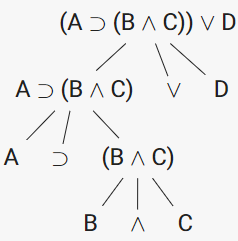
\includegraphics{formula_ad_albero.png}
    \end{center}

    \subsection{Linguaggi formali}
    \begin{itemize}
        \item Un linguaggio si dice \textbf{formale} se rispetta le seguenti proprietà:
        \begin{itemize}
            \item Le formule ed i termini di $L$ sono definiti da formule sintattiche.
            \item Il dominio $D$ denotato da $L$ è formalmente definito.\\
                Chiamiamo $D$ il dominio di interpretazione di $L$.
            \item La denotazione $Den$ di $L$, indicata con $L=Den(D)$ è una funzione:
            \begin{center}
                $I:L \to D$
            \end{center}
            $I$ è chiamata funzione di interpretazione di $L$.
        \end{itemize}
        \item Un linguaggio non formale definito da sintassi formale è chiamato \textbf{linguaggio semi-formale}.
    \end{itemize}

    \section{Linguaggi formali}
    Riprendendo la definizione precedente.
    \begin{itemize}
        \item Un linguaggio si dice \textbf{formale} se rispetta le seguenti proprietà:
        \begin{itemize}
            \item Le formule ed i termini di $L$ sono definiti da formule sintattiche.
            \item Il dominio $D$ denotato da $L$ è formalmente definito.\\
                Chiamiamo $D$ il dominio di interpretazione di $L$.
            \item La denotazione $Den$ di $L$, indicata con $L=Den(D)$ è una funzione:
            \begin{center}
                $I:L \to D$
            \end{center}
            $I$ è chiamata funzione di interpretazione di $L$.
        \end{itemize}
    \end{itemize}

    \subsection{Linguaggi formali con frasi e termini atomici}
    \begin{itemize}
        \item L'interpretazione di un termine è un elemento del dominio.
        \item E' possibile avere sinonimi ma non polisemia.
        \item La funzione simbolica è usata per generare termini complessi.\\
                Viene usata una funzione n-aria che denota lo spazio di tutti i possibili termini che possono essere costruiti. 
        \item Le entità generate da queste funzioni sono tuple (n+1)-arie.
    \end{itemize}

    \subsection{Esempi}
    \subsubsection{1}
    Sia $L$ un linguaggio formale, potrebbe essere eroneamente definito come segue:
    \begin{itemize}
        \item \textbf{Frasi dell'alfabeto} = \{A,B\}
        \begin{itemize}
            \item A = "Fausto ha meno di 25 anni"
            \item B = "Fausto è un professore di IA"
        \end{itemize}
        \item \textbf{Regole di fomrazione delle frasi} = A, B sono le sole formule.
        \item \textbf{D} = \{ $f_1$ = "il fatto cheFausto ha 60 anni", $f_2$ = "il fatto cheFausto è un professore di IA" \}
        \item \textbf{Interpretazione} $I:L \to D$
        \begin{itemize}
            \item $I(A)=???$ $I$ non è una funzione interpretativa di $L$, devo aggiungere fatti o abbandonare $A$.
            \item $I(B)=f_2$
        \end{itemize}
    \end{itemize}

    \subsubsection{2}
    Il linguaggio formale $L$ che prima era sbagliato potrebbe essere ridefinito come:
    \begin{itemize}
        \item \textbf{Frasi dell'alfabeto} = \{A,B\}
        \begin{itemize}
            \item A = "Fausto ha meno di 25 anni"
            \item B = "Fausto è un professore di IA"
        \end{itemize}
        \item \textbf{Regole di fomrazione delle frasi} = A, B sono le sole formule.
        \item \textbf{D} = \{ $f_1$ = "il fatto cheFausto ha 60 anni", $f_2$ = "il fatto cheFausto è un professore di IA", $f_3$ = "il fatto che fausto abbia meno di 25 anni" \}
        \item \textbf{Interpretazione} $I:L \to D$
        \begin{itemize}
            \item $I(A)=f_3$
            \item $I(B)=f_2$
        \end{itemize}
    \end{itemize}

    \subsection{Proposizioni}
    \begin{itemize}
        \item \textbf{Proposizione(secondo Aristotele):} una proposizione è una frase che afferma o nega un predicato.
        \item \textbf{Proposizione:} è una formula che può essere o vera o falsa.
    \end{itemize}

    \subsection{Osservazioni}
    Consideriamo le tre seguenti frasi.
    \begin{enumerate}
        \item A = "Fausto ha meno di 25 anni"
        \item B = "Fausto è un professore di IA"
        \item C = "Fausto ha 60 anni"
    \end{enumerate}
    Possiamo interpretare queste frasi come dei fatti detti $I(A)=f_1$, $I(B)=f_2$, $I(C)=f_3$.\\
    Possiamo anche interpretare il loro valore di verità $I\prime (A)=F$, $I\prime (B)=T$, $I\prime (C)=T$.\\
    Abbiamo cambiato il dominio di interpretazione da $D$ a $D\prime$, quindi dobbiamo anche cambiiare la funzione:
    \begin{center}
        $I:L \to D \Rightarrow I\prime:L \to D^L$
    \end{center}
    Dove $D=\{f\}$ e $D^L$ è un insieme di due distinti valori di proposizioni che stanno per vero, falso.\\
    Riferendoci all'esempio precedente i due domini di interpretazione $D$ e $D^L$ intendono due insiemi molto diveri.
    \begin{enumerate}
        \item $D$ è l'insieme dei fatti che descrivono il mondo.
            \begin{center}
                $D = \{I(A)=f_1, I(B)=f_2, I(C)=f_3\}$
            \end{center}
        \item $D^L$ è l'insieme di giudizi che dicono quali sono i casi nel nostro mondo.
            \begin{center}
                $D^L = \{I\prime(A)=F, I\prime(A)=F, I\prime(B)=F, I\prime(B)=F,I\prime(C)=F, I\prime(C)=F\}$
            \end{center}
    \end{enumerate}
    Il passo tra $D$ e $D^L$ risolve il problema dei domini, possiamo affermare che un fatto certo non può essere casuale.

    \subsection{Linguaggio formale con proposizioni}
    \subsection{Esempio}
    \begin{itemize}
        \item \textbf{Alfabeto} = \{$A$, $B$\}
        \item \textbf{Dominio} D = \{0, 1\}
        \item \textbf{Interpretazione} $I:L \to D$
        \item $\textbf{T}_1$ = \{B\}, $\textbf{T}_2$ = \{A, B\}
        \item $\textbf{M}_1$ = \{I(B)\}, $\textbf{M}_2$ = \{I(A), I(B)\}
    \end{itemize}

    \subsection{Osservazioni}
    Consideriamo l'esempio precedente:
    \begin{itemize}
        \item $L$ = \{A, B\}
        \item $T_1$ =\{B\} $T_2$ = \{A, B\}
        \item $D$ = \{1, 0\}
        \item I1(L) = \{I1(B)=1, I1(A)=0\} = \{I1(B)\}: I1 è un modello $M_1$ di $T_1$ ma non di $T_2$.
        \item I2(L) = \{I2(B)=1, I2(A)=1\} = \{I2(B), I2(A)\}: I2 è un modello $M_2$ di $T_1$ e di $T_2$.
        \item I3(L) = \{I3(B)=0, I3(A)=1\} = \{I3(A)\}: I3 non è un modello $M$ di $T_1$ e $T_2$.
        \item I4(L) = \{I4(B)=0, I4(A)=0\} = $\emptyset$: I4 non è un modello $M$ di $T_1$ né di $T_2$.
    \end{itemize}
    Una teoria viene considerata incompleta/parziale se descrive il vero valore \textbf{di un sotto insieme} di formule atomiche del linguaggio.\\
    Un modello è un interpretazione che soddisfa tutte le formule di una teoria.\\
    Una teoria può avere più modelli.

    \subsection{La negazione}
    Sia $L$ un linguaggio formale, $I:L \to D$ la sua funzione di interpretazione con $D$ = \{0, 1\} e sia $\lnot$ un simbolo primitivo dell'alfabeto allora:
    \begin{itemize}
        \item Se I(A)=1 allora I($\lnot$A)=0
        \item Se I(A)=0 allora I($\lnot$A)=1
    \end{itemize}
    Dove $\lnot$A si legge come "non A".

    \subsection{Osservazione}
    Una teoria $T$ che contiene sia la formula A che $\lnot$A non ha modello e viene detta \textbf{contradditoria}.

    \subsection{Relazione di implicazione}
    Sia $L$ un linguaggio formale, $I:L \to D$ la sua funzione di interpretazione con $D$ = \{0, 1\}, sia $T \subseteq L$ una teoria formale, sia $M \subseteq D$ un modello per $T$ allora $\models_L$ è la funzione di implicazione che associa cosa è vero in $M$ con le wff in $T$.
    \begin{center}
        $\models_L \subseteq M \times T$
    \end{center}
    Possiamo anche scrivere:
    \begin{center}
        $M \models_L T$
    \end{center}
    Dicendo che $M$ implica $T$.

    \subsection{Negazione con implicazione}
    Sia $L$ un linguaggio formale, la funzione di interpretazione $I:L \to D$ \dots\\
    Allora per ogni formula atomica $A \in L$:
    \begin{itemize}
        \item I $\models$ A se I(A)=True
        \item I $\models$ $\lnot$A se non è vero che I $\models$ A (I $\not\models$ A)
    \end{itemize}

    \subsection{Osservazioni}
    \begin{itemize}
        \item Una teoria $T$ che contiene sia la formula A che $\lnot$A non ha modello e viene detta \textbf{contradditoria}.
        \item Per ogni formula A la formula A$\land \lnot$A viene detta \textbf{contraddizione}.
        \item Per ogni formula A la formula A$\lor \lnot$A viene detta \textbf{tautologia}.
    \end{itemize}

    \section{Modello mentale formale}
    \subsection{Nozioni}
    Un modello formale è un modello formale in cui:
    \begin{itemize}
        \item La relaziona tra formule atomiche ed il dominio di interpretazione sono formalizzate da una funzione di interpretazione.
        \item Le relazione tra modello e teoria è formalizzata dalla relazione di implicazione.
    \end{itemize}
    La costruzione di un modello mentale formalizzato segue i seguenti step:
    \begin{enumerate}
        \item Il linguaggio è dato.
        \item Dominio e funzione di interpretazione sono dati.
        \item La funzione di implicazione è data.
        \item Un modello è costruito assumendo che un certo insieme di fatti sia vero.
        \item Ci sono \textbf{solo} 2 usi per un modello formale:
        \begin{enumerate}
            \item \textbf{Modellazione (apprendimento):} il modello formale viene creato/esteso.
            \item \textbf{Ragionamento:} il modello formale viene usato per risolvere delle query.
        \end{enumerate}
    \end{enumerate}
    Un sistema logic-based che ragiona su conoscenze e dati ha due componenti principali:
    \begin{enumerate}
        \item Una conoscenza di base (\textbf{KB}) tale che KB$\subseteq$L che è una teoria del mondo.
        \item Un sistema di ragionamento che risponde alle query grazie al contenuto del KB.
    \end{enumerate}

    \chapter{Teoria degli insiemi}
    \section{Insieme}
    \textbf{Insieme:} una collezione di elementi la cui descrivono deve essere non ambigua ed univoca

    \subsection{Concetti di base}
    \begin{itemize}
        \item \textbf{Insieme vuoto:} è l'insieme che non contiene elementi e si indica $\emptyset$.
        \item \textbf{Appartenenza:} a$\in$A indica che l'elemento a appartiene all'insieme A.
        \item \textbf{Non appartenenza:} è il contrario dell'appartenenza e si indica a$\notin$A.
        \item \textbf{Uguaglianza:} A = B se e solo A e B contengono gli stessi elementi.
        \item \textbf{Non uguaglianza:} se A e B non sono ugualu si indica con A $\neq$ B.
        \item \textbf{Sottoinsieme:} A$\subseteq$B indica che tutti gli elementi di A appartenegono anche a B.
        \item \textbf{Sottoinsieme proprio:} se e solo se A$\subseteq$B e A$\neq$B allora si dice che A$\subset$B.
    \end{itemize}

    \subsection{Power set}
    \textbf{Definizione:} il power set di un insieme è l'insieme contenente tutti i sottoinsiemi di A.


    Se l'insieme ha $n$ elementi il suo power set ha $2^n$ elementi.

    \subsection{Operazioni sugli insiemi}
    \subsubsection{Unione}
    Dati due insiemi A e B la loro unione A$\cup$B è defina come l'insieme di tutti gli elementi appartenenti sia ad A si che B.

    \subsubsection{Intersezione}
    Dati due insiemi A e B definiamo la loro intersezione A$\cap$B come l'insieme che contiene gli elementi che appartengono contemporanemente ad A e a B.

    \subsubsection{Differenza}
    Dati due insiemi A e B la loro differenza A$-$B è l'insieme A a cui sono stati tolti tutti gli elementi che aveva in comune con B.

    \subsubsection{Complemento}
    Dati due insiemi A e B tali che A$\subseteq$B defininiremo il complemenetare di A in B come l'insieme di tutti gli elementi che appartengono a B ma non ad A, lo indicheremo con $\bar{\text{A}}$ oppure $\text{C}_{\text{B}}\text{A}$.

    \subsection{Proprietà delle operazioni}
    Con lo stesso insieme:
    \begin{itemize}
        \item A$\cap$A=A
        \item A$\cup$A=A
    \end{itemize}
    Commutative:
    \begin{itemize}
        \item A$\cap$B=B$\cap$A
        \item A$\cup$B=B$\cup$A
    \end{itemize}
    Con l'insieme vuoto:
    \begin{itemize}
        \item A$\cap \emptyset$=$\emptyset$
        \item A$\cup \emptyset$=A
    \end{itemize}
    Associative:
    \begin{itemize}
        \item (A$\cap$B)$\cap$C=A$\cap$(B$\cap$C)
        \item (A$\cup$B)$\cup$C=A$\cup$(B$\cup$C)
    \end{itemize}
    Dsitributive:
    \begin{itemize}
        \item A$\cap$(B$\cup$C)=(A$\cap$B)$\cup$(A$\cap$C)
        \item A$\cup$(B$\cap$C)=(A$\cup$B)$\cap$(A$\cup$C)
    \end{itemize}
    Leggi di De Morgan:
    \begin{itemize}
        \item $\overline{\text{A} \cup \text{B}}$=$\bar{\text{A}} \cap \bar{\text{B}}$
        \item $\overline{\text{A} \cap \text{B}}$=$\bar{\text{A}} \cup \bar{\text{B}}$
    \end{itemize}

    \subsection{Prodotto cartesiano}
    Dati deu insiemi A e B, definiamo il prodotto cartesiano di A e B come l'insieme delle tuple ordinate (a,b) tali che a$\in$A e b$\in$B.\\
    Formalmente si può esprimere come:
    \begin{center}
        $A \times B=\{(\text{a,b}) : \text{a} \in \text{A and b} \in \text{B}\}$
    \end{center}

    \subsubsection{Oservazioni}
    \begin{itemize}
        \item A$\times$B$\neq$B$\times$A
        \item Il prodotto cartesiano può essere applicato ad $n$ insiemi di insiemi $\text{A}_1$, $\text{A}_2$, \dots , $\text{A}_n$.\\
        $\text{A}_1 \times \text{A}_2 \times \dots \times \text{A}_n$ sarà l'insieme ordinato di n-tuple ($\text{x}_1$, \dots , $\text{x}_n$) dove $\text{x}_i \in \text{A}_i$ per ogni $i=1 \dots n$
    \end{itemize}

    \section{Relazioni}
    \textbf{Definizione:} una relazione R dall'insieme A ad un insieme B è un sottoinsieme del prodotto cartesiano di A e B: R$\subseteq$A$\times$B.


    Se (x,y)$\in$R scriveremo xRy e diremmo "x è R-relazionato a y".


    Una relazione binaria su un insieme A è un sotto insieme R$\subseteq$A$\times$A.
    \spazio
    Data una relazio e R da A a B:
    \begin{itemize}
        \item Il dominio di R è l'insieme $Dom(\text{R})$=\{a$\in$A $|$ esiste un b$\in$B che aRb\}
        \item Il codominio di R è l'insieme $Cod(\text{R})$=\{b$\in$B $|$ esiste un a$\in$A che aRb\}
    \end{itemize}

    \subsection{Relazione inversa}
    Sia R una relazione da A a B, la relazione inversa di R è la relazione $\text{R}^{-1} \subseteq \text{B} \times \text{A}$ definita come:
    \begin{center}
        $\text{R}^{-1}$=\{(b,a) $|$ (a,b)$\in$R\}
    \end{center}

    \subsection{Proprietà delle relazioni}
    Sia R una relazione binaria A, allora R può avere le seguenti proprietà:
    \begin{itemize}
        \item \textbf{Riflessiva:} se e solo se aRa per ogni a$\in$A.
        \item \textbf{Simmetrica:} se e solo se aRb implica che bRa per ogni a,b$\in$A.
        \item \textbf{Transitiva:} se e solo se aRb e bRc implica che aRc per ogni a,b,c$\in$A.
        \item \textbf{Anti-simmetrica:} se e solo se aRb e bRa implica che a=b per ogni a,b$\in$A.
    \end{itemize}

    \subsection{Relazione di equivalenza}
    Sia R una relazione binaria su un insieme A.\\
    R è una relazione di equivalenza se e solo se soddisfa le seguenti proprietà:
    \begin{itemize}
        \item Riflessiva
        \item Simmetrica
        \item Transitiva
    \end{itemize}
    Le relazioni di equivalenza sono spesso indicate con $\sim$ oppure con $\equiv$.

    \subsection{Partizione di insiemi}
    Sia A un insieme , una partizione di A è una famiglia F di sottoinsiemi non vuoti tali che:
    \begin{itemize}
        \item L'unione di tutti i sottoinsiemi sia A.
        \item I sottoinsiemi sono disgiunti a coppie.
    \end{itemize}
    Ogni elemento di A apprtiene esattamente ad un insieme di F.

    \subsection{Classe di equivalenza}
    Sia A un insieme e $\equiv$ una relazione di equivalenza su A, dato x$\in$A definiamo classe di equivalenza  X l'insieme di elementi x$\prime \in$A tale che x$\prime \equiv$x, formalmente:
    \begin{center}
        X=\{x$\prime | $x$\prime \equiv$x\}
    \end{center}
    E' possibile prendere ogni elemento di x per ottenere una classe di equivalenza X, la classe di equivalenza è denotata anche da [x].

    \subsection{Insieme quoziente}
    L'insieme quozienete di A è l'insieme delle classi di equivalenza definite da $\equiv$ su A, denotato da A/$\equiv$

    \subsubsection{Teorema}
    Data una relazione di equivalenza $\equiv$ su A, la classe di equivalenza definita da $\equiv$ su Aè una partizione di A.


    Similmente, data una partizione di A, la relazione R definita come xRx$\prime$ se e solo se x e x$\prime$ appartengono allo stesso sottoinsieme, e una relazione di equivalenza.

    \subsection{Relazione di ordinamento}
    Sia A un insieme e R una relazione binaria su A.


    R è un ordinamento \underline{parziale}, denotato come $\leq$, se:
    \begin{itemize}
        \item \textbf{Riflessiva:} a$\leq$a
        \item \textbf{Anti-simmetrica:} a$\leq$b e b$\leq$a allora a=b.
        \item \textbf{Transitiva:} a$\leq$b e b$\leq$c allora a$\leq$c.
    \end{itemize}
    Se la relazione vale per tutti gli a,b$\in$A allora si dice \underline{ordinamento totale}.\\
    Una relazione è in \underline{ordine stretto}, denotata con $<$, se:
    \begin{itemize}
        \item \textbf{Transitiva:} a$<$b e b$<$c allora a$<$c.
        \item Per ogni a,b$\in$A o a$<$b o b$<$a oppure a=b.
    \end{itemize}

    \section{Funzioni}
    Dati due insiemi A e B, una funzione f da A a B è una relazione che associa ad ogni elemento di a in A esattamente un elemento un elemento b in B, denotata con:
    \begin{center}
        f: A $\to$ B
    \end{center}
    Il dominio di f è tutto l'insieme A.\\
    L'immagine di ogni elemento a in A è l'elemento di b in B tale che b=f(a).\\
    Il codominio di f è un sottoinsiemi di B, definito come segue:
    \begin{center}
        $\text{Im}_\text{f}$=\{b$\in$B $|$ $\exists$ a$\in$A tale che b=f(a)\}
    \end{center}

    \subsection{Classi di funzioni}
    \begin{enumerate}
        \item \textbf{Suriettive:} una funzione f: A $\to$ B è suriettiva se ogni elemento in b è l'immagine di qualche elemento in A.
        \item \textbf{Iniettiva:} una funzione f: A $\to$ B è iniettiva se ogni elemento di A ha un immagine diversa in B.
        \item \textbf{Biettiva:} una funzione f: A $\to$ B è biettiva se è sia iniettiva che suriettiva.
        \item \textbf{Inversa:} se f: A $\to$ B è biettiva possiamo defnire una funzione inversa:
            \begin{center}
                f$^{-1}$: B $\to$ A
            \end{center}
    \end{enumerate}

    \subsection{Funzioni composte}
    Siano f: A $\to$ B e g: B $\to$ C funzioni, allora la composizione di f e g creerà la funzione g$\circ$f: A $\to$ C.
    \begin{itemize}
        \item (g$\circ$f)(a) = g(f(a))
    \end{itemize}

    \chapter{Ragionamento formale}
    \section{Logiche}
    \begin{itemize}
        \item \textbf{Logica:} una logca L è una tripla $\mathcal{L}$=$\langle L, I, \models \rangle$ dove L è un linguaggio formale, I una funzione di interpretazione I: L $\to$ D e $\models$ una relazione di implicazione.
        \item \textbf{Calcolo logico:} un calcolo logico $\mathcal{C}_\mathcal{L}$ è una tupla $\mathcal{C}_\mathcal{L} = \langle \mathcal{L}, \mathcal{P} \rangle$ dove $\mathcal{L}$ è una logica e $\mathcal{P}$ un insieme di domande.
        \item \textbf{Ragionamento logico:} dato un calcolo logico $\mathcal{C}_\mathcal{L}$, con ragionamento logico indichiamo il processo con il quale si risolve un problema applicando un algoritmo non per forza terminale.
    \end{itemize}

    \subsection{Logica proposizionale}
    Le caratteristiche di questa logica sono:
    \begin{itemize}
        \item Un linguaggio proposizionale contiene solo proposizioni primitive.
        \item Le formule sono interpretate attraverso un dominio di giudizi.
        \item Le formule complesse sono formate usando un numero arbitrario di connettivi proposizionali.
        \item I connettivi proposizionali possono essere.
        \begin{itemize}
            \item $\lnot$ letto come "not" per la negazione.
            \item $\land$ letto come "and" per le congiunzioni.
            \item $\lor$ letto come "or" per le disgiunzioni.
            \item $\Longrightarrow$ letto come "implies" per le implicazioni.
            \item $\Longleftrightarrow$ letto come "if and only if" per le equivalenze.
            \item $\uparrow$ letto come "nand" per le congiunzioni negate.
            \item $\downarrow$ letto come "nor" per le disngiunzioni negate.
        \end{itemize} 
    \end{itemize}
    La logica proposizionale è utile per problemi che possono essere formalizzati per essere indipendenti da strutture interne.
    
    \subsection{Logica del primo ordine}
    Le caratteristiche di questa logica sono:
    \begin{itemize}
        \item Termini e formule sono complesse.
        \item Molto spesso le formule primitive non sono parte del linguaggio.
        \item Termini e formule atomiche sono interpretate su un dominio di entità e fatti.\\
            Le formule complesse sono interpretate attraverso un dominio di giudizi.
        \item Le formule complesse sono formate usando connettivi proposizionali e un numero arbitrario di quanificatori.
        \item I quantificatori sono:
        \begin{itemize}
            \item $\forall$ letto come "for all" per quantificare tutti i termini di un insieme.
            \item $\exists$ letto come "there exists" per dire se esiste almeno un elemento in un insieme.
        \end{itemize}
    \end{itemize}
    La logica del primo ordine è utile ogni volta la struttura interna dei termini e la loro composizione per formare la verità o la falsità di una formula atomica è importante, quindi quando è importante essere molto descrittivi.

    \subsection{Logica descrittiva}
    Le caratteristiche di questa logica sono:
    \begin{itemize}
        \item Le logiche proposizionali + una logica del primo ordine permettono di usare solo formule atomiche e non primitive.
        \item Solo predicati unari e binari sono permessi.
        \begin{itemize}
            \item Predicati unari detti classi.
            \item Predicati binari detti ruoli.
        \end{itemize}
        \item Termini e formule sono interpretati su un dominio di entità e fatti.
        \item Le forule complesse sono formate usando connettivi proposizionali e due operatori modali.
        \item Gli operatori modali sono:
        \begin{itemize}
            \item $\exists R$ letto come "there exists an element of \dots" per quantificare l'esistenza su un codominio di ruoli.
            \item $\forall R$ letto come "for all elements of" per la quantificazione universale su un codominio di ruoli.
        \end{itemize}
    \end{itemize}
    I modelli di logica descrittiva permettono di rappresentare e ragionare sui diagrammi ER, diagrammi UML e knowledge graph.

    \section{Problemi di ragionamento}
    Il ragionamento è usato per ultimare alcuni compiti come:
    \begin{itemize}
        \item Verifica del modello.
        \item Soddisfacibilità.
        \item Validità.
        \item Insoddisfacibilità.
        \item Conseguenza logica.
        \item Equivalenza logica.
    \end{itemize}

    \subsection{Tabelle di verità}
    Sono il modo per dimostrare la verità dei fatta oppure di una proposizione che descrive quei fatti.\\
    Permettono di descriveve ogni possibile modello M di un certo dominio D, questo significa costruire ogni possibile combinazione di fatti.\\
    Infatti esistono $2^n$ possibili modelli con $n$ il numero di fatti nel dominio.\\
    Due frasi che rappresentano lo stesso fatto avranno lo stesso valore e possono essere rappresentate da una sola proposizione.
    \subsubsection{Esempi}
    \begin{minipage}{0.33333\textwidth}
        \begin{tabular}{|c|c|c|}
            \hline
            A & B & A$\land$B\\
            \hline
            1 & 1 & 1\\
            \hline
            1 & 0 & 0\\
            \hline
            0 & 1 & 0\\
            \hline
            0 & 0 & 0\\
            \hline
        \end{tabular}
    \end{minipage}
    \begin{minipage}{0.33333\textwidth}
        \begin{tabular}{|c|c|}
            \hline
            A & $\lnot$A\\
            \hline
            0 & 1\\
            \hline
            1 & 0\\
            \hline
        \end{tabular}
    \end{minipage}
    \begin{minipage}{0.33333\textwidth}
        \begin{tabular}{|c|c|c|}
            \hline
            A & B & A$\uparrow$B\\
            \hline
            1 & 1 & 0\\
            \hline
            1 & 0 & 1\\
            \hline
            0 & 1 & 1\\
            \hline
            0 & 0 & 1\\
            \hline
        \end{tabular}
    \end{minipage}

    \subsection{Verifica del modello}
    Data un teoria T e un modello M, la verifica consiste nel verificare che qualsiasi sia M possa essere un modello valido per T, equivale a verificare che M$\models$T.

    \subsection{Soddisfacibilità}
    Una teoria T viene detta soddisfacibile se esiste un modello rappresentato da T, invece se viene dato T bisogna verificare se esiste o meno un modello M che coincide con un modello descritto da T.

    \subsubsection{Esempio}
    Dobbiamo compilare la tabella di verità di A$\land$B per vedere se la formula è soddisfacibile o meno.
    \begin{center}
        \begin{tabular}{|c|c|c|}
            \hline
            A & B & A$\land$B\\
            \hline
            1 & 1 & 1\\
            \hline
            1 & 0 & 0\\
            \hline
            0 & 1 & 0\\
            \hline
            0 & 0 & 0\\
            \hline
        \end{tabular}
    \end{center}
    La formula è soddisfatta visto che c'è almeno un modello che implica la formula, ovvero che è vero.

    \subsection{Validità}
    Una teoria T è detta valida se ogni modello possibile è rappresentato da T.\\
    Una teoria T è detta valida se ogni modello M del nostro dominio soddisfa T, e.g.:
    \begin{center}
        $\forall$M, M$\models$T
    \end{center}

    \subsubsection{Esempio}
    Computiamo ora la tabella di verità di $\lnot$(A$\land \lnot$A) per verificare che la formula sia valida o meno.
    \begin{center}
        \begin{tabular}{|c|c|c|}
            \hline
            A & $\lnot$A & $\lnot$(A$\land \lnot$A)\\
            \hline
            1 & 0 & 1\\
            \hline
            0 & 1 & 1\\
            \hline
        \end{tabular}
    \end{center}

    \subsection{Insoddisfacibilità}
    Una teoria T è detta insoddisfabile se non c'è un modello rappresentato da T.\\
    Una teoria T è detta insoddisfabile se:\\
    Non esiste un modello M tale che
    \begin{center}
        M$\models$T
    \end{center}
    Ogni modello M è tale che:
    \begin{center}
        M$\not \models$T
    \end{center}

    \subsubsection{Esempio}
    Computiamo ora la tabella di verità di A$\land \lnot$A per verificare che la formula sia soddisfabile o meno.
    \begin{center}
        \begin{tabular}{|c|c|c|}
            \hline
            A & $\lnot$A & A$\land \lnot$A\\
            \hline
            1 & 0 & 0\\
            \hline
            0 & 1 & 0\\
            \hline
        \end{tabular}
    \end{center}
    La formula risulta insoddisfabile visto che non ci sono modelli che la implicano.

    \subsection{Conseguenza logica}
    Una teoria $\text{T}_2$ viene detta conseguenza logica di un'altra teoria $\text{T}_1$ se ogni modello rappresentato da $\text{T}_1$ viene rappresentato anche da $\text{T}_2$.
    \begin{center}
        $\forall$M: M$\models$$\text{T}_1$,  M$\models$$\text{T}_2$
    \end{center}

    \subsubsection{Esempio}
    Computiamo ora la tabella di verità di A e $\lnot$($\lnot$A$\land$B$\land$$\lnot$A) per vedere se quest'ultima è una conseguenza di A:
    \begin{center}
        \begin{tabular}{|c|c|c|}
            \hline
            A & B & $\lnot$($\lnot$A$\land$B$\land$$\lnot$A)\\
            \hline
            1 & 1 & 1\\
            \hline
            1 & 0 & 1\\
            \hline
            0 & 1 & 0\\
            \hline
            0 & 0 & 1\\
            \hline
        \end{tabular}
    \end{center}
    Come si può vedere la formula è una conseguenza logica di A visto che ogni volta che A è 1 anche la formula lo è.

    \subsection{Equivalenza logica}
    Una teoria $\text{T}_1$ viene detta equivalenza logica di un'altra teoria $\text{T}_2$ rappresentano lo stesso modello.
    \begin{center}
        $\forall$M: M$\models$$\text{T}_1$ se e solo se M$\models$$\text{T}_2$
    \end{center}

    \subsubsection{Esempio}
    Computiamo ora la tabella di verità di A e $\lnot$($\lnot$A$\land \lnot$(B$\land \lnot$B)) per vedere se le due formule sono logicamente equivalenti.
    \begin{center}
        \begin{tabular}{|c|c|c|}
            \hline
            A & B & $\lnot$($\lnot$A$\land \lnot$(B$\land \lnot$B))\\
            \hline
            1 & 1 & 1\\
            \hline
            1 & 0 & 1\\
            \hline
            0 & 1 & 0\\
            \hline
            0 & 0 & 0\\
            \hline
        \end{tabular}
    \end{center}
    Le formule $\lnot$($\lnot$A$\land \lnot$(B$\land \lnot$B)) e A sono equivalenze logiche visto che sono vere e false negli stessi momenti.

    \section{Scegliere una logica}
    Per affrontare un problema dobbiamo seguire i seguenti passi:
    \begin{enumerate}
        \item Formalizzare le domande e le risposte di un problema.
        \item Sviluppare l'approccio che ci sembra più logico.
        \item Scegliere il tipo di logica più adatto.
        \item Scrivere la teoria T che modella il problema.
        \item Usare la logica per risolvere il problema.
    \end{enumerate}
    Sulla scelta della logica bisogna prestare molta attenzione perchè ogni logica è caratterizzata da:
    \begin{itemize}
        \item \textbf{Diversa espressività} Quali problemi di decione posso esprimere.
        \item \textbf{Efficenza computazionale} Quanto è oneroso risolvere un problema decisionale.
    \end{itemize}

    \subsection{Decidibilità}
    Una logica è decidibile se esiste un metodo efficace per verificare che una formula appartenga sia inclusa in una teoria.
    \begin{itemize}
        \item Il metodo effettivo è un algoritmo che dato un problema decisionale ritorna vero o falso.
        \item Tutte le logiche del corso sono decidibili, tranne la logica del primo ordine.
    \end{itemize}

    \subsection{Complessità}
    Data una logica decidibile la complessità quantifica la difficoltà a computare il ragionamento in una data logica.
    I linguaggi logici sono classificati secondo vari gradi di complessità:
    \begin{itemize}
        \item P
        \item NP
        \item PSpace\\
        \vdots
    \end{itemize}

    \subsection{Espressività}
    \begin{center}
        \begin{tabular}{|c|c|c|}
            \hline
            Linguaggio & Frasi NL & Formule\\
            \hline
            Logica proposizionale & \makecell{Fausto likes skiing\\ I like skiing} & \makecell{Fausto-likes-skiing\\ I-like-skiing}\\
            \hline
            Logica del primo ordine & \makecell{Every person likes skiing\\ I like skiing\\ Fausto likes skiing} & \makecell{$\forall$person.like-skiing(person)\\ like-skiing(I)\\ like-skiing(Fausto)}\\
            \hline
            Logica descrittiva & Every perons likes cars & person $\sqsupseteq \exists$ likes.Car\\
            \hline
        \end{tabular}
    \end{center}

    \chapter{Usare modelli formali}
    \section{Livello di formalizzazione}
    \subsection{Linguaggio specifico}
    Esistono diversi tipi di linguaggi specifici che dipendono dal linguaggio che usano.
    \begin{itemize}
        \item \textbf{Modelli informali} usano linguaggio naturale.
        \item \textbf{Modelli semi-formali} usano lingiiagi strutturati con sintassi semi-formali e delle semantiche informali.
        \item \textbf{Modelli logici} usano linguaggi formali.
    \end{itemize}

    \subsection{Perchè i linguaggi informali?}
    \begin{center}
        \begin{tabular}{|c|c|c|}
            \hline
            Usato per & Vantaggi & Svantaggi\\
            \hline
            Specifiche informali & \makecell{Economico da usare\\ Utile per interagire con utenti} & \makecell{La semantica è informale\\ Impossibile da automatizzare}\\
            \hline
        \end{tabular}
    \end{center}

    \subsection{Perchè i diagrammi?}
    \begin{center}
        \begin{tabular}{|c|c|c|}
            \hline
            Usato per & Vantaggi & Svantaggi\\
            \hline
            Specifiche semi-formali & \makecell{Economico da usare\\ Utile per interagire con utenti} & \makecell{La semantica è informale\\ Impossibile da automatizzare}\\
            \hline
        \end{tabular}
    \end{center}

    \subsection{Perchè le logiche?}
    \begin{center}
        \begin{tabular}{|c|c|c|}
            \hline
            Usato per & Vantaggi & Svantaggi\\
            \hline
            \makecell{Specifiche formali\\ Automazioni} & \makecell{Molto capibile per le sintassi e semantiche formali\\ Molto efficente da automatizzare} & Difficile da usare con gli utenti\\
            \hline
        \end{tabular}
    \end{center}

    \section{Usare le logiche}
    Esempi di problemi:
    \begin{itemize}
        \item Usare una teoria per concordare.
        \item Usare una teoria per garantire l'interoperabilità.
        \item Usare il ragionamento $\models$ per garantire che il programma faccia ciò per cui è pensato.
        \item Usare il ragionamento per implementare IA.
    \end{itemize}
\end{document}